\documentclass[border=0.3cm, 11pt]{standalone}
\usepackage{tikz}
\usepackage{amsmath, amssymb, amsfonts}
\usepackage{color}

\begin{document}
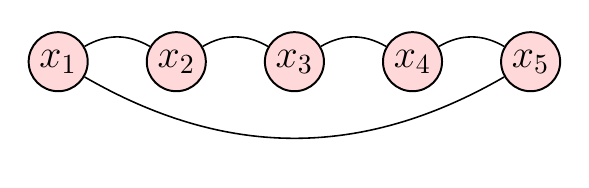
\begin{tikzpicture}

\node[circle, line width = 0.25mm, draw = black, fill = red!15, inner sep = 0pt, minimum size = 0.75cm] (x1) at (0, 0) {\Large${x}_{1}$};
\node[circle, line width = 0.25mm, draw = black, fill = red!15, inner sep = 0pt, minimum size = 0.75cm] (x2) at (1.5, 0) {\Large${x}_{2}$};
\node[circle, line width = 0.25mm, draw = black, fill = red!15, inner sep = 0pt, minimum size = 0.75cm] (x3) at (3, 0) {\Large${x}_{3}$};
\node[circle, line width = 0.25mm, draw = black, fill = red!15, inner sep = 0pt, minimum size = 0.75cm] (x4) at (4.5, 0) {\Large${x}_{4}$};
\node[circle, line width = 0.25mm, draw = black, fill = red!15, inner sep = 0pt, minimum size = 0.75cm] (x5) at (6, 0) {\Large${x}_{5}$};

\path [draw, line width = 0.2mm, -] (x1) edge [bend left] node [right] {} (x2);
\path [draw, line width = 0.2mm, -] (x2) edge [bend left] node [right] {} (x3);
\path [draw, line width = 0.2mm, -] (x3) edge [bend left] node [right] {} (x4);
\path [draw, line width = 0.2mm, -] (x4) edge [bend left] node [right] {} (x5);

\path [draw, line width = 0.2mm, -] (x1) edge [bend right] node [left] {} (x5);

\end{tikzpicture}
\end{document}